\documentclass[a4,useAMS,usenatbib,usegraphicx,12pt]{article}
%External Packages and personalized macros
%=========================================================================
%		EXTERNAL PACKAGES
%=========================================================================
\usepackage[round]{natbib}
\usepackage[margin=3cm]{geometry}
\usepackage{hyperref}
\usepackage{times}
\usepackage{amsmath} 
\usepackage{amssymb}
\usepackage{graphicx}
\usepackage{array, xcolor, bibentry}

\definecolor{lightgray}{gray}{0.8}
\newcolumntype{L}{>{\raggedleft}p{0.14\textwidth}}
\newcolumntype{R}{p{0.8\textwidth}}
\newcommand\VRule{\color{lightgray}\vrule width 0.5pt}

\usepackage{booktabs}% http://ctan.org/pkg/booktabs
\newcommand{\tabitem}{~~\llap{\textbullet}~~}

%=========================================================================
%		INTERNAL MACROS
%=========================================================================
% To highlight comments 
\definecolor{red}{rgb}{1,0.0,0.0}
\newcommand{\red}{\color{red}}
\definecolor{darkgreen}{rgb}{0.0,0.5,0.0}
\newcommand{\SRK}[1]{\textcolor{darkgreen}{\bf SRK: \textit{#1}}}
\newcommand{\SRKED}[1]{\textcolor{darkgreen}{\bf #1}}

\newcommand{\LCDM}{$\Lambda$CDM~}
\newcommand{\beq}{\begin{eqnarray}}  
\newcommand{\eeq}{\end{eqnarray}}  
\newcommand{\zz}{$z\sim 3$} 
\newcommand{\apj}{ApJ}  
\newcommand{\apjs}{ApJS}  
\newcommand{\apjl}{ApJL}  
\newcommand{\aj}{AJ}  
\newcommand{\mnras}{MNRAS}  
\newcommand{\mnrassub}{MNRAS accepted}  
\newcommand{\aap}{A\&A}  
\newcommand{\aaps}{A\&AS}  
\newcommand{\araa}{ARA\&A}  
\newcommand{\nat}{Nature}  
\newcommand{\physrep}{PhR}
\newcommand{\pasp}{PASP}    
\newcommand{\pasj}{PASJ}    
\newcommand{\avg}[1]{\langle{#1}\rangle}  
\newcommand{\ly}{{\ifmmode{{\rm Ly}\alpha}\else{Ly$\alpha$}\fi}}
\newcommand{\hMpc}{{\ifmmode{h^{-1}{\rm Mpc}}\else{$h^{-1}$Mpc }\fi}}  
\newcommand{\hGpc}{{\ifmmode{h^{-1}{\rm Gpc}}\else{$h^{-1}$Gpc }\fi}}  
\newcommand{\hmpc}{{\ifmmode{h^{-1}{\rm Mpc}}\else{$h^{-1}$Mpc }\fi}}  
\newcommand{\hkpc}{{\ifmmode{h^{-1}{\rm kpc}}\else{$h^{-1}$kpc }\fi}}  
\newcommand{\hMsun}{{\ifmmode{h^{-1}{\rm {M_{\odot}}}}\else{$h^{-1}{\rm{M_{\odot}}}$}\fi}}  
\newcommand{\hmsun}{{\ifmmode{h^{-1}{\rm {M_{\odot}}}}\else{$h^{-1}{\rm{M_{\odot}}}$}\fi}}  
\newcommand{\Msun}{{\ifmmode{{\rm {M_{\odot}}}}\else{${\rm{M_{\odot}}}$}\fi}}  
\newcommand{\msun}{{\ifmmode{{\rm {M_{\odot}}}}\else{${\rm{M_{\odot}}}$}\fi}}  
\newcommand{\lya}{{Lyman$\alpha$~}}
\newcommand{\clara}{{\texttt{CLARA}}~}
\newcommand{\rand}{{\ifmmode{{\mathcal{R}}}\else{${\mathcal{R}}$ }\fi}}  


%MY COMMANDS #############################################################
\newcommand{\sub}[1]{\mbox{\scriptsize{#1}}}
\newcommand{\dtot}[2]{ \frac{ d #1 }{d #2} }
\newcommand{\dpar}[2]{ \frac{ \partial #1 }{\partial #2} }
\newcommand{\pr}[1]{ \left( #1 \right) }
\newcommand{\corc}[1]{ \left[ #1 \right] }
\newcommand{\lla}[1]{ \left\{ #1 \right\} }
\newcommand{\bds}[1]{\boldsymbol{ #1 }}
\newcommand{\oiint}{\displaystyle\bigcirc\!\!\!\!\!\!\!\!\int\!\!\!\!\!\int}
\newcommand{\mathsize}[2]{\mbox{\fontsize{#1}{#1}\selectfont $#2$}}
\newcommand{\eq}[2]{\begin{equation} \label{eq:#1} #2 \end{equation}}
\newcommand{\lth}{$\lambda_{th}$ }
%#########################################################################

\setlength\parindent{0pt}
 
\title{Impact of orbital decay and recoil mergers kicks on the growth of SMBHs}
\author{Sebastian Bustamante}
\date{}
  
\begin{document}
\maketitle
\tableofcontents
 
\newpage 

%==================================================================================================
\section{Dynamical friction in SMBHs}
%==================================================================================================



%==================================================================================================
\section{Spin evolution of SMBHs}
%==================================================================================================

The angular momentum of a SMBH is defined by the following expression:

\eq{SpinBH}
{ J_{bh} = |a|\frac{GM_{bh}^2}{c} }

where $a$ is the spin parameter, satisfying the condition $0\leq |a| \leq 1$. This is imposed from
assuming a rotating Kerr BH, where the maximum spin allowed for a BH is $GM_{bh}^2/c$.

\

We assume two main processes through which BHs can be spun up or spun down, namely gas accretion and 
BH-BH binary coalescence. For gas accretion, we model spin evolution of SMBHs by adopting the model 
presented by \citet{Fanidakis2011}.

%--------------------------------------------------------------------------------------------------
\subsection{Modelling gas accretion}
%--------------------------------------------------------------------------------------------------

We assume here that a gas accretion disk is formed around the BH if the mass accretion rate is above 
$1\%$ of the Eddington rate \citep{Fanidakis2011}. For accretion rates below this value, the gas does 
not carry enough angular momentum to modify significantly the spin of the BH. Additionally, we assume
a thin Shakura-Sunyaev disk model \citep{Shakura1973}.

\subsubsection{Spin evolution equation}

Once the accretion disk is set, the orbiting gas loses its angular momentum due to viscous torques
caused by magnetic fields \citep{Lynden-Bell1969}, moving inwards and reaching then the radius of the 
last stable orbit (LSO) of the BH, which can be expressed in terms of the BH's spin \citep{Bardeen1972}:

\eq{LSO}
{ \hat{r}_{lso} = \frac{r_{lso}}{R_g} = 3 + Z_2 \pm [ (3-Z_1)(3+Z_1+2Z_2) ]^{1/2} }

where the negative sign is taken for a counter-rotating BH (i.e. $a<0$) and positive in case of 
co-rotation. Also, for convenience, a normalization with the gravitational radius $R_g$ is used, which 
is defined as half of the Schwarzschild radius:

\eq{Rgrav}
{ R_g = \frac{R_{Schw}}{2} = \frac{GM_{bh}}{c} }

finally, the quantities $Z_1$ and $Z_2$ depend on the BH's spin, and are defined as:

\begin{eqnarray}
Z_1 &\equiv& 1 + (1-a^2)^{1/3}\left[ (1+a)^{1/3} + (1-a)^{1/3} \right] \\
Z_2 &\equiv& ( 3a^2 + Z_1^2 )^{1/2}
\end{eqnarray}

Once the gas reaches the edge of the accretion disk at the LSO, we assumed that is immediately accreted,
adding up to the total BH's mass and angular momentum:

\eq{AccretedMandS}
{ dM_{bh} = \frac{\tilde{e}}{c^2}dM_0,\ \ \ dJ_{bh} = \tilde{l}_{lso}dM_0 }

where $\tilde{e}$ and $\tilde{l}$ are the energy and angular momentum per unit rest mass of the infalling
gas and $dM_0$ the mass of an accreted gas parcel. The differential equation for the evolution of the spin 
can be then derived from the previous expressions, yielding:

\eq{DSpinEvolution}
{ \frac{da}{d \ln M_{bh} } = \frac{1}{M_{bh}}\frac{c^3}{G}\frac{\tilde{l}_{lso}}{\tilde{e}_{lso}} - 2a }

which can be integrated to obtain the final evolution equation \citep{Bardeen1970}:

\begin{eqnarray}
a^f  & = & \frac{1}{3}\hat{r}_{lso}^{1/2}\frac{M_{bh}}{M^f_{bh}}\left[ 1 - \left\{ 3\hat{r}_{lso}\left(\frac{M_{bh}}{M^f_{bh}}\right)^2 - 2 \right\}^{1/2} \right],
    \ \ \ \ \frac{M^f_{bh}}{M_{bh}} \leq \hat{r}_{lso}^{1/2} \\
a^f  & = & 0.998, \ \ \ \ \frac{M^f_{bh}}{M_{bh}} > \hat{r}_{lso}^{1/2}
\end{eqnarray}

where $M^f_{bh}$ and $a^f_{bh}$ are the mass and the spin of the BH after the accretion episode. 
Bardeen's original formula assigns a maximum spin value of $1$ once the final-initial mass ratio is 
above $\tilde{r}_{lso}^{1/2}$, however, following the argument of \citet{Thorne1974}, the accretion 
disk radiates and some of these photons are accreted by the BH. Photons with angular momentum 
opposite to the spin of the BH will then counteract it, thereby reducing the maximum value that can 
be reached, setting an upper limit of $a = 0.998$.

\subsubsection{Accreting gas in misaligned disks}

The previous discussion led us to obtain the formula to calculate spin evolution once a mass $M_b = 
M^f_{bh} - M_{bh}$ is accreted by the BH. However, we still need to estimate this mass. In order to 
do so, we assume the most general situation where a tilted and warped accretion disk forms around
the BH. We define the angular momentum of the BH and the disk as $\bds{J}_{bh}$ and $\bds{J}_{d}$
respectively. The total angular momentum is defined then as:

\eq{TotalJ}
{ \bds J_{tot} = \bds J_{bh} + \bds J_{d} }


due to conservation of angular momentum in the BH-disk system, this vector is constant (magnitude
and orientation) during the whole accretion episode.

In Figure \ref{fig:AccretionDisk} it is defined the relative orientation of the vectors. $\theta$ is 
the angle between the BH and the disk angular momentum and satisfies that $0\leq \theta \leq \pi$.
$\theta = 0$ and $\theta = \pi$ correspond to full alignment and anti-alignment respectively. The 
angle $\theta^t$ is defined as the angle between the BH's spin and the total angular momentum.

Using \ref{eq:TotalJ}, the angle $\theta$ satisfies the next equation:

\[ J^2_{tot} = J^2_{bh} + J^2_{d} = 2J_{bh}J_{d}\cos \theta \]

or

\eq{ThetaEvol}
{ \cos\theta = \frac{J^2_{tot} - J^2_{bh} - J^2_{d}}{2J_{bh}J_{d}} }

In the same way, for $\theta^t$:

\[ J_{bh}\cos\theta^t + J_d\cos(\theta - \theta^t) = J_{tot} \]

\eq{ThetatEvol}
{ J_{bh}\sin{\theta^t} = J_d \sin( \theta - \theta^t ) }

%.........................................................................
%Reference system respect which gravitational recoil velocity is applied
\begin{figure}[htbp]
\centering
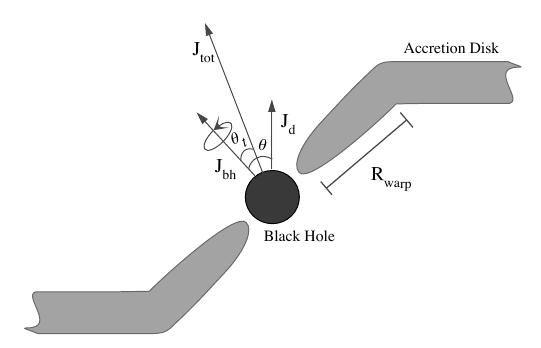
\includegraphics[width=0.6\textwidth]
{./figures/AccretionDisk.png}
\caption{\small{Warped accretion disk around a SMBH. Figure taken from \citet{Fanidakis2011} (Fig 2).}}

\label{fig:AccretionDisk}
\end{figure}
%.........................................................................


Due to the torque caused by the Lense-Thirring effect, the gas around the disk in a misaligned system
will precess around the rotation axis of the BH, and if strong viscosity gradients are present, an 
inner part of the disk will be forced to lay in the equatorial plane of the BH, causing thus an inner 
warped region in the disk (\cite{Fanidakis2011} and references within). The precession rate is given
by \citep{Pringle1992}:

\[ \bds{\Omega}_p = \frac{2G\bds{J}_{bh}}{c^2R^3} \]

From this, the following timescales are defined: the precession timescale $t_{prec}(R)$, viscous 
accretion timescale $t_{\nu_1}(R)$ and warp propagation timescale $t_{\nu_2}(R)$ and , which are 
defined respectively as:

\eq{tpre}
{ t_{prec}(R) \equiv \frac{2\pi}{\Omega_p(R)} }

\eq{Tnu1}
{ t_{\nu_1}(R) \equiv \frac{R^2}{\nu_1(R)} }

\eq{Tnu2}
{ t_{\nu_2}(R) \equiv \frac{R^2}{\nu_2(R)} }


Where $\nu_1$ and $\nu_2$ are the kinematic viscosities acting on velocity gradients parallel and 
perpendicular to the plane of the disk respectively. Following \citet{Volonteri2007}, we adopt $\nu_2
= \nu_1/\alpha^2$ and the Shakura-Sunyaev parameter $\alpha = 0.1$.


In order to estimate the radius of the warped region $R_{warp}$, the timescales for precession and
warp propagation are compared, such that

\[ t_{prec}(R_{warp}) = t_{\nu_2}(R_{warp}) \]

Inside the warp region, we have the condition $t_{prec}\leq t_{\nu_2}$, which means that precession 
is fast enough to avoid viscosity effects propagated in the normal direction to the plane, thereby
keeping the inner region warped. Outside this region, viscosity effects can counteract the deformation.
In terms of the Schwarzschild radius, the warp radius is given by \citep{Volonteri2007}:

\eq{Rwarp}
{ \frac{R_{warp}}{R_{Schw}} = 3.6 \times 10^3 a^{5/8} \left( \frac{M_{bh}}{10^8 M_{\odot}} \right)^{1/8}
\lambda^{-1/4}\left( \frac{\nu_2}{\nu_1} \right)^{-5/8}\alpha^{-1/2} }

where $\lambda \equiv L/L_{Edd}$ is the Eddington ratio.

To estimate the mass accreted by the BH, we assume that the whole mass inside the warp region is 
accreted in the accretion timescale $t_{\nu_1}$, obtaining:

\eq{AccMass}
{ M_d(R_{warp}) = \dot{M} t_{\nu_1}(R_{warp}) }

where $\dot{M}$ is the mass accretion rate of the BH. Using equation \ref{eq:Rwarp}, the accretion 
timescale at the edge of the warp region is:

\eq{AccTimeWarp}
{ t_{\nu_1} = \frac{R^2_{warp}}{\nu_1} = 3\times 10^6 a^{7/8} \left( \frac{M_{bh}}{10^8 M_{\odot}} \right)^{11/8}
\lambda^{-3/4} \left( \frac{\nu_2}{\nu_1} \right)^{-7/8} \alpha^{-3/2}\ yr  }

Finally, we used the alignment condition proposed by \citet{King2005} to evaluate whether the BH is 
aligned or counter-aligned to the accretion disk:

\eq{AlignmentCond}
{ \cos \theta < -\frac{J_d}{2J_{bh}} }

Using the expressions for the Schwarzschild and warp radius, we obtain

\[ \frac{J_d}{2J_{bh}} = 10^{-9} \lambda \left( \frac{t_{\nu_1}}{1\ yr} \right) \left( \frac{R_{warp}}{R_{Schw}} \right)^{1/2}
a^{-1}\]

\subsubsection{Numerical implementation}

The previous formulation of disk accretion by \citet{Fanidakis2011} was based on semi-analytical 
models of galaxy formation, where halos are tracked in the Millenium N-body simulation. Therefore, 
the accretion rate and the total mass budget to feed a BH were estimated semi-analytically from
merger histories. Here instead, we couple in a self-consistent way the spin evolution and the 
numerical outputs for the accretion rate and accreted mass in the AREPO code. The following steps
are followed in the code:

\begin{enumerate}
 \item In cosmological setups, when a fof halo reaches a threshold mass $M_{th}$, a BH is seeded in
 the potential minimum. We initialize the spin of the BH with an initial value $a_{bh,0}$ in a
 random direction. For non-cosmological setups, in the first time-step, the spin of every BH is also
 initialize in the same way. We adopt a conservative value of $a_{bh,0} = 0$, however we will explore
 different choices.
 
 \item Using the BH mass $M_{bh}$, we proceed to calculate the quantities $R_{warp}$, $M_d(R_{warp})$
 and the angular momentum of the disk $J_d(R_{warp})$.
 
 \item A normal vector is drawn for the plane of the accretion disk. This can be done either by 
 randomly draw a vector or by using a parallel vector to the angular momentum of the gas cells used 
 to compute the local density around the BH. This way, we get the initial angles $\theta$ and 
 $\theta^t$. The total angular momentum $\bds J_{tot}$ is also computed in this step, and is kept
 constant during the whole accretion episode.
 


\end{enumerate}






%==================================================================================================
\section{Recoil merger kicks}
%==================================================================================================

%--------------------------------------------------------------------------------------------------
\subsection{Modelling recoils}
%--------------------------------------------------------------------------------------------------

In order to model gravitational recoils of BHs, we used the same approach followed by \citet{Sijacki2009}.
Three different cases of recoils are studied, namely mass asymmetry driven recoils, recoils in 
configurations with arbitrary mass and aligned/anti-aligned spins, and finally, configurations with
arbitrary mass and arbitrary spin orientation. The last case is the most general one and will be the 
approach implemented in the code\footnote{This also means that spin evolution has to be followed in 
the code. It is necessary to learn how to add new properties to a particle type in AREPO.}. In the
following part, the three different approaches are covered in detail.

\subsubsection{Mass asymmetry driven recoils}

In this case, the recoil is purely driven by the mass asymmetry of the two involved BHs. We follow
the Fitchett formula numerically calibrated by \citet{Gonzales2007}:

\eq{Fitchett}
{v_{\mbox{\tiny{m, kick}}} = A \eta^2 \sqrt{ 1 - 4\eta } (1 + B\eta)}

where the parameters $A$ and $B$ are $1.2\times 10^4$ km/s and $-0.93$ respectively, and the parameter
$\eta$ is defined as $\eta = q/(1+q)^2$, with $q = m_1/m_2\leq 1$.

Although the two involved BHs have a null spin, the remnant will acquire a non-zero value due to 
the angular momentum carried away by the gravitational waves (GW). The formula for the spin gained by
the remnant is given by:

\eq{SpinRemnant}
{ a_{\mbox{\tiny{fin}}} = 3.464 \eta - 2.029\eta^2 }

\subsubsection{Configuration with arbitrary mass ratio and aligned/anti-aligned spins}

In this second case, both BHs are allowed to have a spin in the direction of the orbital angular 
momentum of the binary system, either aligned or anti-aligned. In this case, the recoil velocity 
can reach higher values (up to $460$ km/s). The standard formula is given by:

\eq{RecoilAligned}
{ \vec{v}_{\mbox{\tiny{ align, kick }}} = v_{\mbox{\tiny{m, kick}}} \hat{e_1} + 
v_{\bot}( \cos{\xi}\hat{e_1} + \sin{\xi}\hat{e_2} ) }

with 

\eq{PerpendVel}
{ v_{\bot} = H\frac{\eta^2}{1+q}(a_2-qa_1) }

Here, $\hat{e_1}$ and $\hat{e_2}$ are orthogonal vectors lying in the orbital plane. $\xi$ is an 
angle between the unequal mass and spin contribution to kick velocity. Here, it is adopted the value
$\xi = 90^o$. For the parameter $H$, we adopt the same value as in \citet{Campanelli2007}, i.e. 
$H = 7.3 \times 10^3$ km/s.

\subsubsection{Configuration with arbitrary mass ratio and random spin orientation}

For this last case, both BHs are allowed to have an arbitrary mass and a random spin orientation. 
The recoil velocity is then given by the next formula:

\eq{RecoilGeneral}
{ \vec{v}_{\mbox{\tiny{ align, kick }}} = v_{\mbox{\tiny{m, kick}}} \hat{e_1} + 
v_{\bot}( \cos{\xi}\hat{e_1} + \sin{\xi}\hat{e_2} ) + v_{\parallel}\hat{e_z} }

where

\eq{ParallVel}
{ v_{\parallel} = K \cos( \Theta - \Theta_0 )\frac{\eta^2}{1+q}( a_2^{\bot} - qa_1^{\bot} ) }

Here, $K = 6\times 10^4$ km/s, $\Theta_0 = 0.184$. $\Theta$ is defined as the angle between 
the in-plane component of the vector $\vec{\Delta} = (m_1+m_2)(\vec{a_1}-\vec{a_2})$ and the infall 
direction at the merger, which is taken as the radial direction just before the coalescence. In figure
\ref{fig:RecoilReferenceSystem} we show the reference system used to apply the recoil velocity to the
remnant.

%.........................................................................
%Reference system respect which gravitational recoil velocity is applied
\begin{figure}[htbp]
\centering
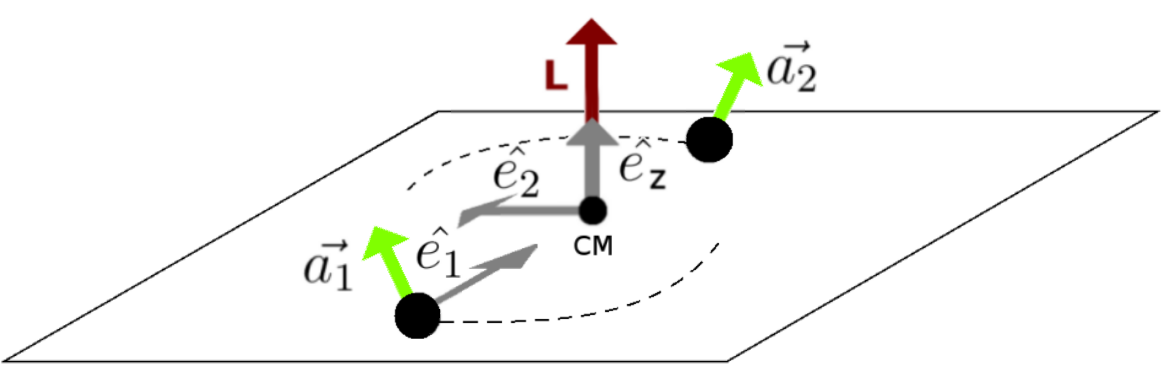
\includegraphics[width=0.7\textwidth]
{./figures/BinarySystem.png}
\caption{\small{Reference system that is used to apply the recoil velocity of the BH remnant.}}

\label{fig:RecoilReferenceSystem}
\end{figure}
%.........................................................................

We also correct for the eccentricity of the orbit using the formula proposed by \citep{Sopuerta2007}:

\eq{CorrectionEcc}
{ \vec{v}_{e} = \vec{v}_{\mbox{\tiny{ align, kick }}}( 1+e ) }

This approach is the most general one and will be implemented in our study.


%--------------------------------------------------------------------------------------------------
\subsection{Numerical implementation}
%--------------------------------------------------------------------------------------------------

In order to adapt the previous scheme to our simulations, we adopt a series of assumptions that 
facilitates the numerical implementation, namely:

\begin{itemize}
 \item Only merger events involving two BHs take place in the simulation. Three-BHs merger events
 are split up in two two-BHs mergers.
 \item The two BHs will merge once they are closer than the minimum of the softening lengths used to 
 compute the gas density for each BH.
 \item They will merge irrespectevely of their approach velocity. Usually, a criterion based on the
 local speed of sound would provide a more realistic scenario, however, as a first-order estimative,
 we do not apply this.
 \item The reference system used in the estimation of the kick velocity is built based on the
 state of the system just before the numerical coalescence. This clearly differs from the physical 
 coalescence as the binary system should take some time before the merger event, which happens after 
 the distance becomes less than smoothing length. However, this scale is by no means, well-resolved 
 in our simulations, so we neglect this time. We also assume that the angular momentum is not 
 significantly changed during the coalescence phase and the orbital plane, which defines our recoil 
 system, can be taken as the same in the numerical coalescence.
 \item Spin evolution is not considered here (at the moment). We assume that BHs accrete mass in a 
 chaotic and episodic way, as proposed by \citet{King2008}. This accretion mode regularize the spin
 of the BH as the infalling matter does not contribute constructively to spin up the BH. The random 
 and chaotic nature of the accretion makes the spin quickly converge to a value of $a = 0.3 \pm 0.2$.
\end{itemize}


\subsubsection{Setting up the spins}

Merger events are the only processes that can significantly spin up a BH, however the spin of the 
remnant should be quickly slowed down by chaotic and episodic gas accretion in a presumably short 
time scale, thereby erasing any ́"memory" of the initial conditions or the last merger \citep{King2008}. 
Instead of following spin evolution, we set up a random oriented spin for each BH prior to a merger.
The magnitude of the spin parameter is generated based on a normal distribution with $\bar{a} = 0.3$ 
and $2\sigma = 0.2$.

%.........................................................................
%Spin distribution
\begin{figure}[htbp]
\centering
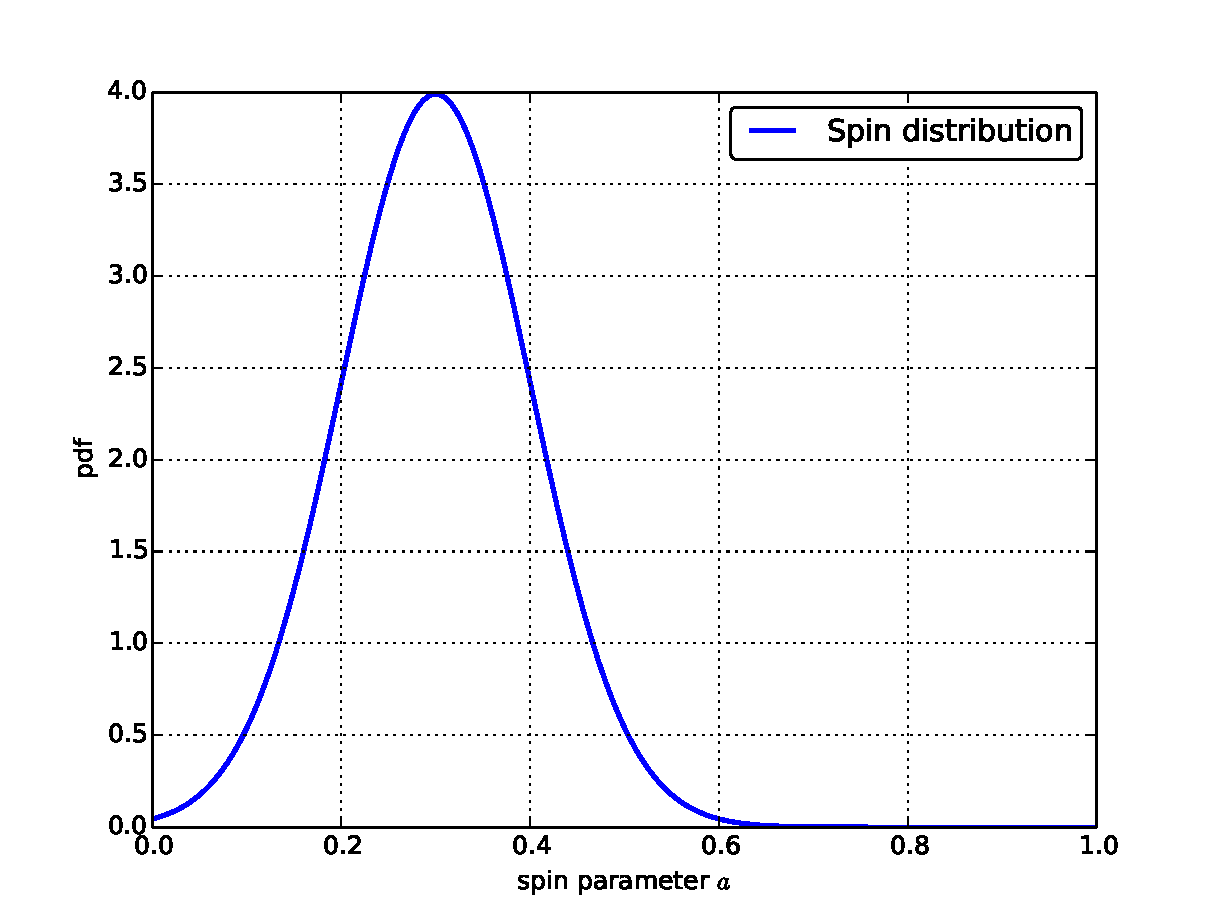
\includegraphics[width=0.50\textwidth]
{./figures/SpinDistribution.pdf}
\caption{\small{Spin distribution function to generate initial values prior to a merger.}}

\label{fig:SpinDistribution}
\end{figure}
%.........................................................................

\subsubsection{Defining reference system}

Prior to the merger, we have the next information from the two involved BHs: $m_1$, $\vec{r_1}$, 
$\vec{v_1}$, $m_2$, $\vec{r_2}$, $\vec{v_2}$ along with the two randomly generated spins $\vec{a_1}$
and $\vec{a_2}$. From this information, we proceed to construct the reference system where the recoil
merger kick will be referred. The respective two-body variables are then $\vec{r} = \vec{r_1} - 
\vec{r_2}$ and $\vec{v} = \vec{v_1} - \vec{v_2}$. The angular momentum of the binary is $\vec{L} = 
\vec{r}\times\vec{v}$. We define the orthonormal system $\hat{e_1}$, $\hat{e_2}$, $\hat{e_z}$ as 
$\hat{e_1} = \vec{r}/r$, $\hat{e_z} = \vec{L}/L$ and $\hat{e_2} = \hat{e_z}\times\hat{e_1}$

%==================================================================================================
\newpage
\bibliographystyle{latex/mn2e}
\renewcommand{\bibname}{8\ \ \ \ Bibliography}
\small
\bibliography{references.bib}
%==================================================================================================



\end{document}
